% Copyright 2010 by Stefano Maggiolo and Nicola Pagani

\documentclass{amsart}

\usepackage[english]{babel}
\usepackage{amssymb}
\usepackage{hyperref}
\usepackage{tikz}
\usepackage{booktabs}
\usepackage{multirow}
\usepackage{mathtools}
\usetikzlibrary{patterns}

\newcommand{\arXiv}[1]{\href{http://arxiv.org/abs/#1}{arXiv:#1}}

\theoremstyle{plain}
\newtheorem{theorem}{Theorem}[section]
\newtheorem{proposition}[theorem]{Proposition}
\newtheorem{corollary}[theorem]{Corollary}
\newtheorem{lemma}[theorem]{Lemma}
\theoremstyle{definition}
\newtheorem{remark}[theorem]{Remark}
\newtheorem{example}[theorem]{Example}
\newtheorem{definition}[theorem]{Definition}
\newtheorem{notation}[theorem]{Notation}


\DeclareMathOperator{\bN}{\mathbb{N}}
\DeclareMathOperator{\mult}{mult}
\DeclareMathOperator{\MAX}{max}
%\DeclareMathOperator{\min}{min}

\newcommand{\graph}{\mathcal{G}}
\newcommand{\abs}[1]{\left|#1\right|}
\newcommand{\ubar}[1]{\underline{#1}}
\newcommand{\obar}[1]{\overline{#1}}
\newcommand{\psm}[1]{\left(\begin{smallmatrix}#1\end{smallmatrix}\right)}

\title{Generating stable modular graphs}
\author{Stefano Maggiolo}
\author{Nicola Pagani}
\date{\today}

\begin{document}

\begin{abstract}
  We present the program \texttt{boundary}, whose source files are
  available at \href{http://people.sissa.it/~maggiolo/boundary/}
  {\texttt{http://people.sissa.it/\~{}maggiolo/boundary/}}. Given two
  natural numbers $g$ and $n$ satisfying $2g+n-2>0$, the program
  generates all genus $g$ stable graphs with $n$ marked points. Each
  such graph determines the topological type of a nodal stable curve
  of arithmetic genus $g$ with $n$ marked points. Our motivation comes
  from the fact that the boundary of the moduli space of stable genus
  $g$, $n$-pointed curves can be stratified by taking loci of curves
  of a fixed topological type.
\end{abstract}

\maketitle
\setcounter{tocdepth}{1}
\tableofcontents



\section{Introduction}

Moduli spaces of smooth algebraic curves have been defined and then
compactified in algebraic geometry by Deligne and Mumford in their
seminal paper~\cite{delignemumford}. A conceptually important
extension of this notion in the case of pointed curves was introduced
by Knudsen \cite{knudsen}.

The points in the boundary of the moduli spaces of pointed, nodal
curves with finite automorphism group. These curves are called
\emph{stable curves} (or pointed stable curves). The topology of one
such curve is encoded in a combinatorial object, called \emph{stable
  graph}.  The boundary of the moduli space admits a topological
stratification, whose elements are curves with a fixed topological
type and a prescribed assignment of the marked points on each
irreducible component.

The combinatorics of the stable graphs have been investigated in
several papers in algebraic geometry, for many different purposes (see
for instance~\cite{modularoperads,opstall,opstall2,stephanie2}). Our
aim with this program is to provide a useful and effective tool to
generate all the stable graphs of genus $g$ with $n$ marked points up
to isomorphism, for low values of $g$ and $n$.

We construct an algorithm to generate all the stable graphs of genus
$g$ with $n$ unordered marked points. The algorithm uses the software
\texttt{nauty}~(\cite{nauty}) to eliminate isomorphic graphs from the
list of graphs thus created. Since to check that two stable graphs are
isomorphic is computationally onerous, we try to generate a low number
of stable graphs, provided that we want at least one for every
equivalence class. The algorithm generates recursively the vectors of
genera, marked points, and the adjacency matrix. While it fills these
data, it checks the stability condition and the condition on the total
genus as early as possible, in order to minimize the time spent on the
branches of the recursion that do not lead to stable graphs. Some
analysis of the algorithm's performances can be seen in
Section~\ref{sec:performance}.

Programs for enumerative computations on
$\overline{\mathcal{M}}_{g,n}$ have been implemented in both Maple and
Macaulay2~(\cite{faber,stephanie1,smith}). Our program can be used,
for example, to improve the results of~\cite[Section 5]{stephanie2},
or to prove combinatorial results on the moduli space of pointed
stable curves with low genus (cfr.~\cite{busonero}, for example
Corollary~5.3).



\section{What to generate}

From now on, we fix two natural numbers $G$ and $N$ such that $2
G-2+N>0$.  For every $K \in \bN^+$, we define $\ubar{K} = \{0, \dots,
K-1\}$. Let $\Sigma_K$ be the symmetric group on the set $\ubar{K}$.

\begin{definition}
  \mbox{}
  \begin{itemize}
  \item An \emph{undirected multigraph\/} $\graph$ is a couple $(V,
    E)$ with $V$ a finite set of \emph{vertices\/} and $E$ a finite
    multiset of \emph{edges\/} with elements in $V \times V/\Sigma_2$.
  \item The multiplicity of $(v, w)$ in $E$ is denoted by $\mult(v,
    w)$.
  \item The \emph{total multiplicity\/} of $\graph$, or its
    \emph{number of edges}, is $\abs{E}$: the cardinality of $E$ as a
    multiset.
  \item The \emph{degree\/} of a vertex $v$ is $\deg v \coloneqq 2
    \mult(v, v) + \sum_{w \neq v} \mult(v, w)$.
  \item A \emph{colored undirected multigraph\/} is a multigraph with
    some additional data attached to each vertex.
  \end{itemize}
\end{definition}

\begin{definition}\label{def:stable graph}
  A \emph{stable graph\/} of type $(G, N)$ is a colored undirected
  multigraph $\graph = (V, E)$, subject to the following conditions.
  \begin{enumerate}
  \item The color of a vertex $v$ is given by a pair of natural
    numbers $(g_v, n_v)$. The two numbers are called respectively the
    \emph{genus} and the \emph{number of marked points} of the vertex
    $v$.
  \item\label{it:condition connected} $\graph$ is connected.
  \item\label{it:condition genus} Its \emph{total genus}, defined as
    $\sum_{v \in V} g_v + \abs{E} - (\abs{V} - 1)$, equals $G$.
  \item Its \emph{total number of marked points}, defined as $\sum_{v
      \in V} n_v$, equals $N$.
  \item\label{it:condition stability} Stability condition: $\deg v +
    n_v \geq 3$ for every vertex $v$ with $g_v = 0$.
  \end{enumerate}
\end{definition}

\begin{notation}
  The number $\deg v + n_v$ is often called the \emph{number of half
    edges} associated to the vertex $v$. It is the number of edges
  that connect $v$ to another vertex plus the number of marked points
  of $v$. Condition \ref{it:condition stability} can be rephrased in:
  for every vertex $v$ of genus $0$, its number of half edges is at
  least $3$.
  %In Section \ref{sec:ranges} we will also use the following terminology:
  %the number of half edges
\end{notation}

Two stable graphs $\graph = (V, E, g, n)$ and $\graph^\prime =
(V^\prime, E^\prime, g^\prime, n^\prime)$ are \emph{isomorphic\/} if
there is a bijection $f\colon V \to V^\prime$ such that:
\begin{itemize}
\item $\mult(v, w) = \mult(f(v), f(w))$ for every $v, w \in V$;
\item $g_v = g^\prime_{f(v)}$ and $n_v = n^\prime_{f(v)}$ for every $v
  \in V$.
\end{itemize}
Our task is to generate one stable graph for each isomorphism class.

\begin{remark}
  Note that from the definition just given, we are working with an
  unordered set of marked points. The output of the program are the
  boundary strata of the moduli space of stable, genus $g$ curves with
  $n$ unordered points $\overline{\mathcal{M}}_{g,n}/ \Sigma_n$.
\end{remark}



\section{Description of the algorithm}\label{sec:description}

In this section we describe the general ideas of our algorithm. Let us
first introduce the notation we use in the program.

\begin{notation}\label{not:gnla}
  The set of vertices $V$ will always be $\ubar{K}$, so that vertices
  will be identified with natural numbers $i, j, \dots$. The
  multiplicity of the edge between $i$ and $j$ will be denoted by
  $a_{i,j}$: the symmetric matrix $a$ is called the \emph{adjacency
    matrix} of the stable graph. For convenience, we will denote $l_j
  \eqqcolon a_{j,j}$: it is the vector whose elements are the loops at
  the vertex $j$. For simplicity, we will consider $g_j$, $n_j$,
  $l_j$, $a_{i,j}$ to be defined also for $i$ or $j$ outside
  $\ubar{K}$, in which case their value is always assumed to be $0$.
\end{notation}

\begin{remark}
  In the following, we assume $\abs{V} > 1$ in order not to deal with
  degenerate cases. There are trivially $G+1$ stable graphs of type
  $(G, N)$ with one vertex. Indeed, if there is exactly one vertex,
  the choice of the genus uniquely determines the number of loops on
  it after Definition~\ref{def:stable graph}.
\end{remark}

The program uses recursive functions to generate the data that
constitute a stable graph. In order, it generates the numbers $g_j$,
then the numbers $n_j$, $l_j$ (the diagonal part of the matrix $a$),
and finally, row by row, a symmetric matrix representing $a$.

When all the data have been generated, it tests that all the
conditions of Definition~\ref{def:stable graph} hold, in particular
that the graph is actually connected and satisfies the stability
conditions. Then it uses the software \texttt{nauty}~\cite{nauty} to
check if this graph is isomorphic to a previously generated graph. If
this is not the case, it adds the graph to the list of graphs of genus
$G$ with $N$ marked points.

% The program follows two principles: the first is to generate the
% smallest possible number of couples of isomorphic stable graphs, the
% second is to check the conditions of Definition~\ref{def:stable
%   graph} as early as possible, to minimize the time spent in
% branches that do not lead to stable graphs.

% The range is computed in such a way that assigning a value
% outside the range would not generate any stable graph; moreover, we
% tried to minimize the situations in which assigning a value inside
% the range would not generate any stable graph.  We will describe in
% details the ranges in Section~\ref{sec:ranges}.

% Now let us focus on \underline{the first principle}.

A priori, for each entry of $g$, $n$, $l$, and $a$ the program tries
to fill that position with all the integers. This of course is not
possible, indeed it is important to observe here that each datum is
bounded. From below, a trivial bound is $0$, that is, no datum can be
negative. Instead, a simple upper bound can be given for each entry of
$g$ by the number $G$, and for each entry of $n$ by the number
$N$. For $l$ and $a$, upper bounds are obtained from $G$ using the
condition on the total genus (Condition~\ref{def:stable graph}).

These bounds are coarse: Section \ref{sec:ranges} will be devoted to
proving sharper bounds, from above and from below. Also, we will make
these bounds dynamical: for instance assigning the value $g_0 > 0$
clearly lowers the bound for $g_j, j > 0$. In any case once we know
that there are bounds, we are sure that the recursion terminates.

The algorithm follows the following principle: we want to generate the
smallest possible number of couples of isomorphic stable graphs. Here
we generalize the idea that to generate a vector for every class of
vectors of length $K$ modulo permutations, the simplest way is to
generate vectors whose entries are increasing. The program fills the
data row by row in the matrix:
\begin{equation}\label{eq:big matrix}
  \begin{pmatrix}
    g_0 & g_1 & \cdots & g_{K-1}\\
    n_0 & n_1 & \cdots & n_{K-1}\\
    l_0 & l_1 & \cdots & l_{K-1}\\
    \hline
    \bullet & a_{0,1} & \cdots & a_{0,K-1}\\
    a_{1,0} & \bullet & \ddots & \vdots\\
    \vdots & \ddots & \bullet & a_{K-2,K-1}\\
    a_{K-1,0} & \cdots & a_{K-1,K-2} & \bullet
  \end{pmatrix}\text{,}
\end{equation}
and generates only matrices whose columns are ordered. Loosely
speaking, we mean that we are ordering the columns lexicographically,
but this requires a bit of care, for two reasons:
\begin{itemize}
\item the matrix $a$ needs to be symmetric; in the program we generate
  only the strictly upper triangular part;
\item the diagonal of $a$ need not be considered when deciding if a
  column is greater than or equal to the previous one.
\end{itemize}

Therefore, to be precise, we define a relation (\emph{order}) for
adjacent columns. Let us call $c_{j-1}$ and $c_j$ two adjacent columns
of the matrix~\eqref{eq:big matrix}. They are said to be equivalent if
$c_{j-1,i} = c_{j,i}$ for any $i \notin \{j-1+3, j+3\}$. If they are
not equivalent, denote with $i_0$ the minimum index such that $i_0
\notin \{ j-1+3, j+3\}$ and $c_{j-1,i_0} \neq c_{j,i_0}$. Then we
state the relation $c_{j-1} < c_j$ if and only if $c_{j-1,i_0} <
c_{j,i_0}$. We do not define the relation for non-adjacent columns.
We say that the data are ordered when the columns are weakly
increasing, that is if, for all $j$, either $c_{j-1}$ is equivalent to
$c_j$ or $c_{j-1} < c_j$.

To ensure that the columns are ordered (in the sense we explained
before), the program keeps track of \emph{divisions}. We start filling
the genus vector $g$ in a non decreasing way, and every time a value
$g_j$ strictly greater than $g_{j-1}$ is assigned, we put a division
before $j$.
% TODO: the following needs to be rewritten
This means that, when assigning the value of $n_j$, we allow
the algorithm to start again from $0$ instead of $n_{j-1}$, because the column
$c_j$ is already bigger than the column $c_{j-1}$.
% Otherwise, if there is not a division before $i$, we would have been
% forced to put a value which is bigger or equal than the one in
% position $i-1$.

After completing $g$, we start filling the vector $n$ in such a way
that, within two divisions, it is non decreasing. Again we introduce a
division before $j$ every time we assign a value $n_j$ strictly
greater than $n_{j-1}$. We follow this procedure also for the vector
$l$.

Finally, we start filling the rows of the matrix $a$. Here the
procedure is a bit different. Indeed even if for the purpose of
filling the matrix it is enough to deal only with the upper triangular
part, imposing the conditions that the columns are ordered involves
also the lower triangular part. A small computation gives that the
value of $a_{i,j}$ is assigned starting from:
\[
\begin{cases}
  0 & \text{if there are divisions before $i$ and $j$}\\
  a_{i,j-1} & \text{if there is a division before $i$ but not before
    $j$}\\
  a_{i-1,j} & \text{if there is a division before $j$ but not before
    $i$}\\
  \max\{a_{i,j-1}, a_{i-1,j}\} & \text{if there are no divisions
    before $i$ or $j$,}
\end{cases}
\]
and we put a division before $i$ if $a_{i,j} > a_{i-1,j}$ and a
division before $j$ if $a_{i,j} > a_{i,j-1}$.

We cannot conclude immediately that this procedure gives us all
possible data up to permutations as in the case of a single
vector. This is because the transformation that the whole matrix
undergoes when a permutation is applied is more complicated: for the
first three rows (the vectors $g,n,l$), it just permutes the columns,
but for the remaining rows, it permutes both rows and columns. Indeed,
to prove that the procedure of generating only ordered columns does
not miss any stable graph is the content of the following section.



\section{The program generates all graphs}\label{sec:proof}

We want to prove the following result.

\begin{proposition}\label{prop:main}
  The algorithm described in the previous section generates at least
  one graph for every isomorphism class of stable graphs.
\end{proposition}

From now on, besides $G$ and $N$, we also fix the number of vertices
$K$, and focus on proving that the algorithm generates at least one
graph for every isomorphism class of stable graphs with $K$ vertices.

% Moreover, in the previous section we proved that all the constraints
% we put on $g$, $n$, $l$, $a$ (apart from the one coming from
% divisions) are justified by the fact if we assign a value outside
% those constraints, the graph we obtain has no hope of becoming
% stable once completed. As a consequence, for simplicity we can prove
% Proposition~\ref{prop:main} assuming that the algorithm uses only
% the divisions constraints.

\begin{notation}
  We have decided previously to encode the data of a stable graph in a
  $(K+3 \times K)$ matrix $G \coloneqq (g, n, l, a)$
  (cfr.~\eqref{eq:big matrix}). We denote by $\mathcal{A}$ the set of
  all such matrices, and by $\mathcal{M}$ the set of all $(K+3 \times
  K)$ matrices that are generated by the algorithm described in the
  previous section.
\end{notation}

We can assume that the graphs generated by the algorithm are stable,
since we explicitly check connectedness and stability. In other words,
we can assume the inclusion $\mathcal{M} \subset \mathcal{A}$. Hence,
in order to prove Proposition~\ref{prop:main}, we will show that every
$G \in \mathcal{A}$ is in $\mathcal{M}$ up to applying a permutation
of $\ubar{K}$. The idea is to give a characterization
(Lemma~\ref{lemma:char}) of the property of being an element of
$\mathcal{M}$.

Recall first that the algorithm generates only matrices whose columns
are ordered as described in Section~\ref{sec:description}. More
explicitly, if $G = (g, n, l, a) \in \mathcal{A}$, then $G \in
\mathcal{M}$ if and only if:
\begin{multline*}
  \forall (i,j)\colon
  i \not\in \{j-1, j\},\\
  \begin{aligned}
    g_{j-1} &> g_j &&\text{does not happen,}\\
    n_{j-1} &> n_j &\Rightarrow\  & g_{j-1} < g_j\,\text{,}\\
    l_{j-1} &> l_j &\Rightarrow\  & g_{j-1} < g_j \vee n_{j-1} < n_j\,\text{, and}\\
    a_{i,j-1} &> a_{i,j} &\Rightarrow\ & g_{j-1} < g_j \vee n_{j-1} < n_j \vee l_{j-1} < l_j \vee\\
    &&&\ \exists i^\prime < i: i^\prime \not\in \{j-1,j\} \wedge a_{i^\prime,j-1} < a_{i^\prime,j}\,\text{.}
  \end{aligned}
\end{multline*}

Let us call a piece of data $g_j$, $n_j$, $l_j$, or $a_{i,j}$ a
\emph{breaking position\/} if it does not satisfy the condition
above. Observe that a matrix $G \in \mathcal{A}$ has a breaking
position if and only if $G$ is not an element of $\mathcal{M}$.

We now introduce a total order on the set $\mathcal{A}$ of matrices $G
= (g,n,l,a)$. If $G$ is such a matrix, let $v(G)$ be the vector
obtained by juxtaposing the vectors $g$, $n$, $l$ and the rows of the
upper triangular part of $a$. For example, if
\[
  G = \begin{pmatrix}
    0 & 0 & 2 & 0\\
    1 & 1 & 0 & 1\\
    0 & 0 & 0 & 0\\
    \hline
    \bullet & 1 & 1 & 1\\
    1 & \bullet & 2 & 1\\
    1 & 2 & \bullet & 0\\
    1 & 1 & 0 & \bullet
  \end{pmatrix}
\]
(with the same structure as~\eqref{eq:big matrix}), then we define
\[
v(G) := (0, 0, 2, 0,\quad 1, 1, 0, 1,\quad 0, 0, 0, 0,\quad 1, 1,
1,\quad 2, 1,\quad 0)\,\text{.}
\]

\begin{definition}\label{def:order}
  If $G, H \in \mathcal{A}$, we write $G \prec H$ if and only if
  $v(G)$ is smaller than $v(H)$ in the lexicographic order.  In this
  case we say that the matrix $G$ is smaller than the matrix $H$.
\end{definition}

Note that this total order on the set of matrices must not be confused
with the partial order described in
Section~\ref{sec:description}. From now on we will always refer to the
latter order on $\mathcal{A}$.

\begin{notation}
  If $\sigma \in \Sigma_K$ is a permutation and $G = (g, n, l, a)$ is
  a graph, then we can apply $\sigma$ to the entries of the data of
  $G$, obtaining an isomorphic graph. The action of $\sigma$ on $G$
  is: $(g,n,l,a)\to (g^\prime,n^\prime,l^\prime,a^\prime)$ where
  $g^\prime_j=g_{\sigma(j)}$, $n^\prime_j=n_{\sigma(j)}$,
  $l^\prime_j=l_{\sigma(j)}$ and $a^\prime_{i,j} =
  a_{\sigma(i),\sigma(j)}$. We denote this new matrix by $\sigma
  G$. We write $\sigma_{i,j}$ for the element of $\Sigma_K$ that
  corresponds to the transposition of $i, j \in \ubar{K}$.
\end{notation}

Now we are able to state the characterization we need to prove
Proposition~\ref{prop:main}.

\begin{lemma}\label{lemma:char}
  Let $G \in \mathcal{A}$; then $G \in \mathcal{M}$ if and only if $G$
  is minimal in the set
  \[
  \bigl\{ \sigma_{j-1,j} G \,\mid\, 0<j<K \bigr\}\text{.}
  \]
  with respect to the order given in Definition~\ref{def:order}.
\end{lemma}

\begin{proof}
  We will prove that $G$ is not minimal if and only if there is a
  breaking position.

  Assume there is at least one breaking position in $G$. If there is
  one in $g$, $n$, or $l$, it is trivial to see that transposing that
  index with the previous one gives a smaller matrix. If this is not
  the case, let $a_{i,j}$ be a breaking position such that
  $a_{i^\prime,j}$ is not a breaking position whenever $i^\prime < i$
  (the position $(i,j)$ is the first breaking position of its
  column). We deduce that $g_{j-1} = g_j$, $n_{j-1} = n_j$, $l_{j-1} =
  l_j$, and that for all $i^\prime < i$ not in $\{j-1,j\}$, we have
  $a_{i^\prime, j-1} = a_{i^\prime, j}$. Let $H \coloneqq
  \sigma_{j-1,j} G$; the vectors $g$, $n$, and $l$ (the first three
  rows) coincide in $G$ and $H$;
  % instead, to explain what changes in
  % $a$, let us distinguish two cases, depicted in Figure~\ref{fig:a}.
  \begin{itemize}
  \item If $j > i$, the smallest breaking position is in the upper
    triangular part of $a$; it is then clear that $H \prec G$.
  \item If $j < i$, the smallest breaking position is in the lower
    triangular part; by using the symmetry of the matrix $a$ again we
    obtain $H \prec G$ (see the right part of Figure~\ref{fig:a}).
  \end{itemize}

  \begin{figure}[t]
    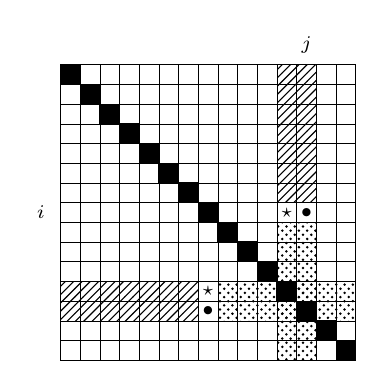
\begin{tikzpicture}[xscale=0.25,yscale=-0.25]
      \node at (-1,7.5) {$\scriptstyle{i}$};
      \node at (12.5,-1) {$\scriptstyle{j}$};
      \node at (11.5,7.5) {$\scriptstyle{\star}$};
      \node at (12.5,7.5) {$\scriptstyle{\bullet}$};
      \node at (7.5,11.5) {$\scriptstyle{\star}$};
      \node at (7.5,12.5) {$\scriptstyle{\bullet}$};
      \fill [pattern=crosshatch dots] (8,11) -- (8,13) -- (15,13) -- (15,11) -- cycle;
      \fill [pattern=crosshatch dots] (11,8) -- (13,8) -- (13,15) -- (11,15) -- cycle;
      \fill [pattern=north east lines] (0,11) -- (0,13) -- (7,13) -- (7,11) -- cycle;
      \fill [pattern=north east lines] (11,0) -- (13,0) -- (13,7) -- (11,7) -- cycle;

      \draw (0,0) -- (15,0) -- (15,15) -- (0,15) -- cycle;
      \foreach \x in {1,2,...,14}
      {
        \draw [very thin] (0,\x) -- (15,\x);
        \draw [very thin] (\x,0) -- (\x,15);
      }
      \foreach \x in {0,1,...,14}
      \filldraw (\x,\x) -- (\x,\x+1) -- (\x+1,\x+1) -- (\x+1,\x) -- cycle;
    \end{tikzpicture}
    \hspace{1.5cm}
    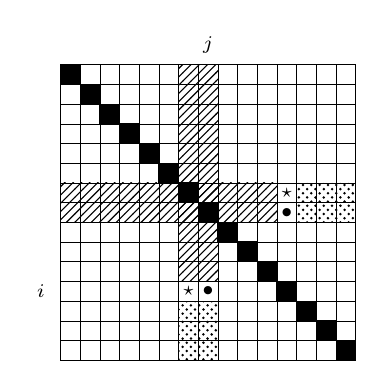
\begin{tikzpicture}[xscale=0.25,yscale=-0.25]
      \node at (-1,11.5) {$\scriptstyle{i}$};
      \node at (7.5,-1) {$\scriptstyle{j}$};
      \node at (6.5,11.5) {$\scriptstyle{\star}$};
      \node at (7.5,11.5) {$\scriptstyle{\bullet}$};
      \node at (11.5,6.5) {$\scriptstyle{\star}$};
      \node at (11.5,7.5) {$\scriptstyle{\bullet}$};
      \fill [pattern=crosshatch dots] (12,6) -- (12,8) -- (15,8) -- (15,6) -- cycle;
      \fill [pattern=crosshatch dots] (6,12) -- (8,12) -- (8,15) -- (6,15) -- cycle;
      \fill [pattern=north east lines] (0,6) -- (0,8) -- (11,8) -- (11,6) -- cycle;
      \fill [pattern=north east lines] (6,0) -- (8,0) -- (8,11) -- (6,11) -- cycle;

      \draw (0,0) -- (15,0) -- (15,15) -- (0,15) -- cycle;
      \foreach \x in {1,2,...,14}
      {
        \draw [very thin] (0,\x) -- (15,\x);
        \draw [very thin] (\x,0) -- (\x,15);
      }
      \foreach \x in {0,1,...,14}
      \filldraw (\x,\x) -- (\x,\x+1) -- (\x+1,\x+1) -- (\x+1,\x) -- cycle;
    \end{tikzpicture}
    \caption{The matrix $a$ when the first breaking position (the
      bullet) is $a_{i,j}$ with $j > i$ (left) or $j < i$
      (right). When transposing $j-1$ and $j$, the white and the
      diagonal-filled entries do not change.}\label{fig:a}
  \end{figure}

  Conversely, let $j$ be such that $H \coloneqq \sigma_{j-1,j} G \prec
  G$. Then consider the first entry (reading from left to right) of
  the vector $v(G)$ that is strictly bigger than $v(H)$. This is a
  breaking position. If it occurs in the matrix $a$ (equivalently, in
  the last $K$ rows), it is actually the smallest breaking position of
  its column.
\end{proof}

% If the first difference between $G$ and $H$ lies in $g$, $n$, or
% $l$, then it is easy to see that the corresponding position is
% breaking. Otherwise, if the three vectors ($g$, $n$, and $l$) of $G$
% and $H$ coincide, let us compare $v(G)$ and $v(H)$, and take the
% first element (reading from left to right)

% we observe Figure~\ref{fig:a} imagining that it
% represents the matrix $a$ for the graph $G$.
% let us compare $a_{i^\prime,j-1}$ and $a_{i^\prime,j}$ for
% $i^\prime = 0$:
% \begin{itemize}
% \item if $a_{0,j-1} > a_{0,j}$, then $a_{0,j}$ is indeed a breaking
%   position for $G$ and we finish;
% \item $a_{0,j-1} < a_{0,j}$ cannot happen, because this would mean
%   that $G \prec H$;
% \item if $a_{0,j-1} = a_{0,j}$, we repeat this trichotomy for
%   $i^\prime = 1$.
% \end{itemize}
% Now, if we iterate the procedure, we continue until $i^\prime =
% j-2$, when we change strategy, comparing instead $a_{j-1,i^\prime}$
% with $a_{j,i^\prime}$, for $i^\prime > j$. The idea is then the
% same: there is a trichotomy, one case conclude our proof, the second
% cannot happen and the third force us to continue. But we cannot
% continue till the end, because if we find always equality, this
% means that $H \not\prec G$, because they are indeed equal.

% \begin{corollary}
%   Given a graph $G$, the number of graphs isomorphic to $G$ that our
%   program generates is bounded by $\abs{\Sigma_K}/(K-1) = K\cdot
%   (K-2)!$.
% \end{corollary}

The proof of Proposition~\ref{prop:main} follows arguing as in this
example.

\begin{example}
  Let $G_0 = G \in \mathcal{A}$ be the graph of the previous example:
  \[
  G_0 = \psm{
    0 & 0 & 2 & 0\\
    1 & 1 & 0 & 1\\
    0 & 0 & 0 & 0\\[2pt]
    \hline\\[1pt]
    \bullet & 1 & 1 & 1\\
    1 &\bullet & 2 & 1\\
    1 & 2 & \bullet & 0\\
    1 & 1 & 0 & \bullet
  }\text{.}
  \]
  This graph is stable but not in $\mathcal{M}$ because, for example,
  $g_2 > g_3$ implies that $g_3$ is a breaking position. Thus we apply
  the permutation $\sigma_{2,3}$, obtaining the graph
  \[
  G_1 \coloneqq \sigma_{2,3} G_0 = \psm{
    0 & 0 & 0 & 2\\
    1 & 1 & 1 & 0\\
    0 & 0 & 0 & 0\\[2pt]
    \hline\\[1pt]
    \bullet & 1 & 1 & 1\\
    1 & \bullet & 1 & 2\\
    1 & 1 & \bullet & 0\\
    1 & 2 & 0 & \bullet
  } \prec G_0\text{.}
  \]
  Now $a_{3,2}$ is a breaking position; applying $\sigma_{1,2}$, we
  obtain
  \[
  G_2 \coloneqq \sigma_{1,2} G_1 = \psm{
    0 & 0 & 0 & 2\\
    1 & 1 & 1 & 0\\
    0 & 0 & 0 & 0\\[2pt]
    \hline\\[1pt]
    \bullet & 1 & 1 & 1\\
    1 & \bullet & 1 & 0\\
    1 & 1 & \bullet & 2\\
    1 & 0 & 2 & \bullet
  } \prec G_1\text{.}
  \]
  This introduces a new breaking position at $a_{3,1}$, so we apply
  the transposition $\sigma_{0,1}$:
  \[
  G_3 \coloneqq \sigma_{0,1} G_2 = \psm{
    0 & 0 & 0 & 2\\
    1 & 1 & 1 & 0\\
    0 & 0 & 0 & 0\\[2pt]
    \hline\\[1pt]
    \bullet & 1 & 1 & 0\\
    1 & \bullet & 1 & 1\\
    1 & 1 & \bullet & 2\\
    0 & 1 & 2 & \bullet
  } \prec G_2\text{.}
  \]
  The graph $G_3$ is finally in $\mathcal{M}$ and indeed no
  transposition can make it smaller.
\end{example}

\begin{proof}[Proof of Proposition~\ref{prop:main}]
  Recall that we have to prove that for every $G \in \mathcal{A}$,
  there is a permutation $\sigma \in \Sigma_K$ such that $\sigma G \in
  \mathcal{M}$.

  So, let $G_0 = G \in \mathcal{A}$. If $G \in \mathcal{M}$, then we
  are done; otherwise, $G$ does not satisfy the condition of
  Lemma~\ref{lemma:char}, hence there is a transposition $\sigma_{j-1,
    j}$ such that $G_1 = \sigma_{j-1,j} G_0 \prec G_0$.

  The iteration of this process comes to an end (that is, we arrive to
  a matrix in $\mathcal{M}$) since the set
  \[
  \bigl\{ \sigma G \mid \sigma \in \Sigma_K\bigr\}
  \]
  is finite.
\end{proof}



\section{Description of the ranges}\label{sec:ranges}

In the previous section we have introduced the algorithm, by
describing the divisions. In this section we introduce accurate ranges
for the possible values of $g,n,l$ and $a$. In particular we try to
obtain estimates on the upper extremum for each datum to be filled.

We will deduce from the conditions of Definition~\ref{def:stable
  graph} some other necessary conditions that can be checked before
the graph is defined in its entirety. More precisely, every single
datum is assigned trying all the possibilities within a range that
depends upon the values of $G$ and $N$, and upon the values of the
data that have already been filled.

The order in which we assign the value of the data is $g$,$n$,$l$, and
finally the upper triangular part of $a$ row after row.

%\begin{notation}
%  At any time during the algorithm, we let $e^{\MAX}$ be the maximum
%  number of edges that could be placed after that time, and $c$ be the
%  number of couples of (different) vertices already connected by an
%  edge. We let $p_1$ be the number of vertices $i$ to which the
%  algorithm has assigned $g_i = 0$. Note that the final value of $p_1$
%  is determined when the first genus greater than $0$ is assigned, in
%  particular the final value of $p_1$ is determined at the end of the
%  assignment of the values to the vector $g$.
%\end{notation}

\begin{notation}
  Suppose we are assigning the $i$-th value of one of the vectors
  $g,n$ or $l$, or the $(i,j)$-th value of $a$. We define the
  following derived variables $e^{\MAX}$, $c$ and $p_1$ that depend
  upon the values that have already been assigned to $g,n,l,a$.

  We let $e^{\MAX}$ be the maximum number of edges that could be
  introduced in the subsequent iterations of the recursion, and $c$ be
  the number of couples of (different) vertices already connected by
  an edge. We let $p_1$ be the number of vertices $z$ to which the
  algorithm has assigned $g_z = 0$.  Note that the final value of
  $p_1$ is determined when the first genus greater than $0$ is
  assigned, in particular the final value of $p_1$ is determined at
  the end of the assignment of the values to the vector $g$.  On the
  other hand, $c$ starts to change its value only when the matrix $a$
  begins to be filled.

  After the assignment of the $i$-th value, the derived values
  $e^{\MAX}$, $c$ and $p_1$ are then updated according to the
  assignment itself.
\end{notation}

\begin{notation} \label{not:partial_assign}
  When deciding $g$, $n$, or $l$, we let $n^{(2)}_i$ be the minimum
  between $2$ and the number of half edges already assigned to the
  $i$-th vertex. This is justified by the fact that we know that at
  least one half edge will be assigned to the $i$-th vertex to connect
  it to the rest of the graph. Hence, whenever $g_i = 0$, $n^{(2)}_i$
  is the number of \emph{stabilizing\/} half edges at the vertex $i$:
  one half edge is needed to connect the vertex to the rest of the
  graph, and then at least two more half edges are needed to stabilize
  the vertex. When deciding $a_{i,j}$, it is also useful to have
  defined $h_i$, the total number of half edges that hit the $i$-th
  vertex. Finally, we define
  \begin{align*}
    G_i &\coloneqq \sum_{i^\prime < i} g_{i^\prime}\,\text{,} &
    N_i &\coloneqq \sum_{\substack{i^\prime < i}} n_{i^\prime}\,\text{,}\\
    N^{(2)} &\coloneqq \sum_{g_{i^\prime} = 0} n^{(2)}_{i^\prime}\,\text{,} &
    N^{(2)}_i &\coloneqq \sum_{\substack{i^\prime < i\\g_{i^\prime} = 0}} n^{(2)}_{i^\prime}\,\text{;}\\
    L_i &\coloneqq \sum_{i^\prime < i} l_{i^\prime}\,\text{,} &
    A_{i,j} &\coloneqq \sum_{\mathclap{i^\prime < i \vee j^\prime < j}} a_{i^\prime, j^\prime}\,\text{.}
  \end{align*}
\end{notation}

We are now ready to describe the ranges in which the data can vary.
We study subsequently the cases of $g$, $n$, $l$ and $a$, thus
following the order of the recursions of our algorithm. Each range is
described by presenting a first list of general constraints on the
parameters and then by presenting a second list containing the actual
ranges in the last line.


\subsection{Range for $g_i$}

When the algorithm is deciding the value of $g_i$, we have the
following situation:
\begin{itemize}
\item $e^{\MAX} = G - G_i + K - 1$ by Condition~\ref{it:condition
    genus};
\item amongst the $e^{\MAX}$ edges, there are necessarily $K-1$
  non-loop edges (to connect the graph); these $K-1$ edges give one
  half edge for each vertex, whereas we can choose arbitrarily where
  to send the other $K-2$ half edges; conversely, the $2(e^{\MAX} - K
  +1)$ half edges of the remaining edges can be associated to any
  vertex; therefore, the maximum number of half edges (not counting
  those that are needed to connect the graph) is $2e^{\MAX} - K + N =
  2(G - G_i) + K - 2 + N$;
  % \item the maximum number of half edges coming from marked points
  %   is $N$;
\item we need $2p_1$ half edges to stabilize the genus $0$ vertices,
  since one half edge comes for free from the connection of the graph.
\end{itemize}

We use the following conditions to limit the choices we have for
$g_i$:
\begin{enumerate}
\item since $g$ is the first vector to be generated, there is no
  division before $i$, hence
  \[
  g_i \geq g_{i-1}\text{;}
  \]
  remember that $g_j = 0$ whenever $j \not\in \ubar{K}$;
\item we need at least $K-1$ non-loop edges, hence (using the fact
  that $\sum_{j \geq i} g_j \geq (K-i) g_i$)
  \begin{align*}
    &e^{\MAX} \geq K-1\\
    &\quad\Rightarrow G - G_i - (K-i) g_i + K-1 \geq K-1\\
    &\quad\Rightarrow (K-i)g_i \leq G - G_i\,\text{;}
  \end{align*}
\item in order to stabilize the $p_1$ vertices of genus $0$ (using the
  fact that one stabilizing half edge comes for free by connection) we
  must have
  \begin{align*}
    &2 p_1 \leq 2e^{\MAX} - K + N\\
    &\quad\Rightarrow 2p_1 \leq G - G_i - (K-i)g_i - K + N\\
    &\quad\Rightarrow (K-i)g_i \leq G - G_i - K + N - 2p_1\,\text{.}
  \end{align*}
\end{enumerate}



\subsection{Range for $n_i$}

When deciding $n_i$, we have the following situation:
\begin{itemize}
\item as before, $e^{\MAX} = G - G_K + K - 1 \geq K-1$, and the
  maximum number of half edges still to be assigned is $2e^{\MAX} - K
  + N - N_i - n_i = 2(G - G_K) + K - 2 + N - N_i - n_i$;
  % \item the number of half edges still to be assigned and coming
  %   from marked points is $N - N_i - n_i$;
\item we need $2p_1 - N^{(2)}_i - n^{(2)}_i$ half edges to stabilize
  the first $p_1$ vertices;
\item if $g_i = 0$, we need $2(i+1) - N^{(2)}_i - n^{(2)}_i$ more half
  edges to stabilize the first $i+1$ vertices.
\end{itemize}

The following conditions define then the ranges for the possible
choices for $n_i$:

\begin{enumerate}
\item if there is not a division before $i$ (that is, if $g_i =
  g_{i-1}$), then we require $n_i \geq n_{i-1}$; otherwise, just $n_i
  \geq 0$;
\item we cannot assign more than $N$ marked points, hence (where we
  treat the case of $g_i = 0$ in a special way)
  \begin{align*}
    &N_i + n_i \leq N\\
    &\quad\Rightarrow n_i \leq N - N_i\\
    &\quad\Rightarrow (p_1 - i)n_i \leq N - N_i\text{ if moreover $g_i = 0$.}
  \end{align*}
\item if $g_i = 0$, for the purpose of stabilizing the first $i+1$
  curves we cannot use marked points anymore, therefore we have
  \begin{align*}
    &2 (i+1) - N^{(2)}_i - n^{(2)}_i \leq (2(G - G_K) + K - 2)\\
    &\quad\Rightarrow n^{(2)}_i = \min(2, n_i) \geq - (2(G - G_K) + K - 2) + (2(i+1) - N^{(2)}_i)\\
    &\quad\Rightarrow
    \begin{cases}
      \text{impossible} & \text{if $\mathrm{RHS} > 2$}\\
      n_i \geq \mathrm{RHS} & \text{otherwise.}
    \end{cases}
  \end{align*}
\end{enumerate}



\subsection{Range for $l_i$}

When deciding $l_{i}$, this is the situation:
\begin{itemize}
\item $e^{\MAX} = G - G_K - L_i - l_i + K - 1 \geq K-1$, and the
  maximum number of half edges still to assign is $2e^{\MAX} - K = 2(G
  - G_K - L_i - l_i) + K - 2$;
\end{itemize}

The conditions on $l_i$ are then the following:
\begin{enumerate}
\item if there is not a division before $i$, then we require $l_i \geq
  l_{i-1}$; otherwise, just $l_i \geq 0$;
\item we need at least $K-1$ non-loop edges, hence
  \begin{align*}
    &e^{\MAX} \geq K-1\\
    &\quad\Rightarrow G - G_K - L_i - l_i + K-1 \geq K-1\\
    &\quad\Rightarrow l_i \leq G - G_K - L_i\,\text{;}
  \end{align*}
\item let $z$ be the index of the genus $0$ vertex with the least
  number of stabilizing half edges such that $z < i$; it already has
  $n_z + 2l_z$ half edges, but we cannot use loops anymore to
  stabilize it; hence,
  \begin{align*}
    &\max(0, 2-n_z-2l_z) \leq G - G_K - L_i - l_i + K - 1\\
    &\quad\Rightarrow l_i \leq G - G_K - L_i + K - 3 + n_z + 2l_z
  \end{align*}
\item assume $g_i = 0$; if $l_i > 0$, we are adding to the $i$-th
  vertex $2-n^{(2)}_i$ stabilizing half edges, and to stabilize the
  $p_1$ genus $0$ vertices, we need to have
  \begin{align*}
    &2 p_1 - N^{(2)} - (2-n^{(2)}_i) \leq 2e^{\MAX} - K\\
    &\quad\Rightarrow 2p_1 - N^{(2)} - (2-n^{(2)}_i) \max(0, 2-m_i) \leq 2(G - G_K - L_i - l_i + K - 1) - K\\
    &\quad\Rightarrow 2l_i \leq 2(G - G_K - L_i) + K + N^{(2)} - n^{(2)}_i - 2p_i\,\text{.}
  \end{align*}
\item assume $g_i = 0$; after deciding $l_i$, we still have $e^{\MAX}$
  edges to place, and each of them can contribute with one half edge
  to the stabilization of the $i$-th vertex; moreover, one of these
  half edges is already counted for the stabilization; hence
  \begin{align*}
    &n_i + 2l_i + (e^{\MAX} - 1) \geq 2\\
    &\quad\Rightarrow n_i + 2l_i + G - G_K - L_i - l_i + K - 1 - 1 \geq 2\\
    &\quad\Rightarrow l_i \geq 4 - n_i - G + G_K + L_i - K\,\text{.}
  \end{align*}
\end{enumerate}



\subsection{Range for $a_{i,j}$}

When deciding $a_{i,j}$, this is the situation:
\begin{itemize}
\item earlier in Notation \ref{not:partial_assign}, we observed that
  for the purpose of filling the vectors $g$,$n$ and $l$ we could
  consider a genus $0$ vertex stabilized when it had at least two
  half-edges (since the graph is going to be connected
  eventually). When assigning the values of $a$, the stability
  condition goes back to its original meaning, i.e. each vertex has at
  least $3$ half edges.
	% This is necessary here since we may have already assigned some
  % non-loop edges, and it would not be easy to keep track of which of
  % the vertices are already connected to the rest of the graph;
\item $e^{\MAX} = G - G_K - L_K - A_{i,j} + K - 1$;
\item we have already placed edges between $c$ couples of different
  vertices;
\end{itemize}

Here are the constraints that $a_{i,j}$ must satisfy:
\begin{enumerate}
\item if there is not a division before $i$, then we require $a_{i,j}
  \geq a_{i-1,j}$; otherwise, just $a_{i,j} \geq 0$;
\item if there is not a division before $j$, then we require $a_{i,j}
  \geq a_{i,j-1}$;
\item we need at least $K-2-c$ (if positive) edges to connect the
  graph, because if $a_{i,j} > 0$, $c$ will increase by $1$ (this
  estimate could be very poor, but enforcing the connectedness
  condition in its entirety before completing the graph is too slow),
  hence:
  \begin{align*}
    &e^{\MAX} - a_{i,j} \geq \max(0, K-2-c)\\
    &\quad\Rightarrow a_{i,j} \leq G - G_K - L_K - A_{i,j} +K - 1 - \max(0, K-2-c)\,\text{;}
  \end{align*}
\item $a_{i,j}$ contributes with at most $\max(0, 3-h_i) + \max(0,
  3-h_j)$ stabilizing half edges; hence, to stabilize the $p_1$ genus
  $0$ vertices, we need
  \begin{align*}
    &3p_1 - \sum_{g_{i^\prime} = 0} \min(3, n_i + 2l_i) - (\max(0, 3-h_i) + \max(0, 3-h_j)) \leq 2 (e^{\MAX} - a_{i,j})\\
    &\quad\Rightarrow 3p_1 - \sum_{g_{i^\prime} = 0} \min(3, n_i + 2l_i) - (\max(0, 3-h_i) + \max(0, 3-h_j)) \leq \\
    &\quad\quad\quad \leq 2 (G - G_K - L_K - A_{i,j} + K - 1 - a_{i,j})\\
    &\quad\Rightarrow 2a_{i,j} \leq 2 (G - G_K - L_K - A_{i,j} + K - 1) - 3p_1 +\\
    &\quad\quad\quad +\sum_{g_{i^\prime} = 0} \min(3, n_i + 2l_i) + \max(0, 3-h_i) + \max(0, 3-h_j)\,\text{.}
  \end{align*}
\item if $j = K-1$ (that is, if this is the last chance to add half
  edges to the $i$-th vertex), then we add enough edges from $i$ to
  $K-1$ in order to stabilize the vertex $i$; moreover, if up to now
  we did not place any non-loop edge on the vertex $i$, we impose
  $a_{i,K-1} > 0$.
  \begin{align*}
    a_{i,K-1}&>0  &&\text{ if $ a_{i,j} = 0$ forall $1<j<K-1$,}\\
    a_{i,K-1}&\geq 3-h_i &&\text{ if $g_i = 0$.}
  \end{align*}
\end{enumerate}



\section{Performance}\label{sec:performance}

The complexity of the problem we are trying to solve is intrinsically
higher than polynomial, because already the amount of data to generate
increases (at least) exponentially with the genera and the number of
marked points. We also observed an exponential growth of the ratio
between the time required to solve an instance of the problem and the
number of graphs generated. Anyway, our program is specifically
designed to attack the problem of stable graphs, and it can be
expected to perform better than any general method to generate graphs
applied to our situation.

We present here some of the results obtained by testing our program on
an Intel\textregistered{} Core\texttrademark 2 Quad Processor Q9450 at
2.66\,GHz. The version we tested is not designed for parallel
processing, hence it used only one of the four cores available.

However, when computing a specific graph, the program needs to keep in
the memory only the graphs with the same values in the vectors $g$,
$n$, $l$. This allows us to neglect memory usage, but also shows that
we can assign the computations of stable graphs with prescribed $g$,
$n$, $l$ to different cores or \textsc{cpu}s, thus having a highly
parallelized implementation of the program.

\begin{figure}[t]
  \includegraphics{plot.pdf}
  \caption{Logarithm of time needed to compute all stable graphs of
    type $(G, N)$.}\label{fig:plot}
\end{figure}

\begin{table}[t]
  \begin{tabular}{rrrr}
    $G$ & $N$ & Time (s) & \# stable graphs\\
    \hline
    0 & 18 & 392 &   847,511\\
    1 & 14 & 539 & 1,832,119\\
    2 & 10 & 147 & 1,282,008\\
    3 &  7 & 117 & 1,280,752\\
    4 &  5 & 459 & 2,543,211\\
    5 &  3 & 606 & 2,575,193\\
    6 &  1 & 226 &   962,172\\
    7 &  0 & 681 & 1,281,678
  \end{tabular}\vspace{\baselineskip}
  \caption{For small $G$, the maximum $N$ such that all stable graphs of type $(G,N)$ can be computed in less than $15$ minutes.}\label{tab:number}
\end{table}

In Table~\ref{tab:number} we list, for each genus $G$, the maximum
number of marked points $N$ for which we can compute all the stable
graphs of type $(G, N)$ under 15 minutes.

In Figure~\ref{fig:plot} we show all the couples $(G, N)$ that we
computed against the time needed; the lines connect the results
referring to the same genus. From this plot it seems that, for fixed
$G$, the required time increases exponentially with $N$. However, we
believe that in the long run the behaviour will be worse than
exponential.

More benchmarks and up-to-date computed results are available
at \texttt{boundary}'s webpage,
\href{http://people.sissa.it/~maggiolo/boundary/}
{\texttt{http://people.sissa.it/\~{}maggiolo/boundary/}}.

\begin{thebibliography}{2}

\bibitem [BMS] {busonero}
  S.~Busonero, M.~Melo, and L.~Stoppino,
  \emph{On the complexity group of stable curves},
  \arXiv{0808.1529}.%v1

\bibitem [DM] {delignemumford}
  P.~Deligne and D.~Mumford,
  \emph{The irreducibility of the space of curves of given genus},
  Inst. Hautes \'Etudes Sci. Publ. Math. \textbf{36} (1969), 75--109.

\bibitem [F] {faber}
  C.~Faber,
  \emph{Maple program for computing Hodge integrals},
  available at \href{http://math.stanford.edu/~vakil/programs/}
  {\texttt{http://math.stanford.edu/\~{}vakil/programs/}}.

\bibitem[GK] {modularoperads}
  E.~Getzler and M.~Kapranov,
  \emph{Modular Operads},
  Compositio Math. \textbf{110} (1998), no. 1, 65--126
  [\arXiv{dg-ga/9408003}].

\bibitem [K]{knudsen}
   F.~Knudsen,
  \emph{Projectivity of the moduli space of stable curves II. The stacks $\overline{M}_{g,n}$}, Math. Scand. \textbf{52} (1983), 161--199.

\bibitem [M] {nauty}
  B.~D.~McKay,
  \emph{nauty},
  available at \href{http://cs.anu.edu.au/people/bdm/nauty/}
  {\texttt{http://cs.anu.edu.au/people/bdm/nauty/}}.

\bibitem [vOV1] {opstall}
  M.~A.~van~Opstall and R.~Veliche,
  \emph{Maximally symmetric stable curves},
  Michigan Math. J. \textbf{55} (2007), no. 3, 513--534
  [\arXiv{math/0603061}].

\bibitem [vOV2] {opstall2}
  M.~A.~van~Opstall and R.~Veliche,
  \emph{Maximally symmetric stable curves II},
  \arXiv{math/0608799}.%v1

\bibitem [SY] {smith}
  G.~Smith and S.~Yang,
  \emph{HodgeIntegral. Macaulay2 package for computing Hodge Integrals},
  available by request from author \href{mailto:stpyang@math.kth.se}
  {\texttt{stpyang@math.kth.se}}.

\bibitem [Y1] {stephanie1}
  S.~Yang,
  \emph{Maple program for computing integrals on $\overline{M}_{g,n}$},
  available by request from author \href{mailto:stpyang@math.kth.se}
  {\texttt{stpyang@math.kth.se}}.

\bibitem [Y2] {stephanie2}
  S.~Yang,
  \emph{Calculating intersection numbers on moduli spaces of pointed curves},
  \arXiv{0808.1974}.%v2

\end{thebibliography}
\end{document}
